\documentclass{UVKABoA4}

\usepackage{graphicx} % Standardpaket zur Grafikeinbindung
\usepackage{amsmath,amssymb} % Erweiterung des Mathematik-Modus
\usepackage{caption}
\usepackage[colorinlistoftodos, english]{todonotes} % Option 'disable' entfernt alle ToDos
\usepackage[absolute,overlay]{textpos}
\usepackage{vmargin}          % Adjust margins in a simple way
\usepackage{tikz}
\usepackage{indentfirst}

% Toggle the following two lines to switch between english and german layout
% \usepackage[english]{babel} % Neue deutsche Rechtschreibung und Silbentrennung.
\usepackage[british, UKenglish, USenglish, english, american]{babel} % Neue deutsche Rechtschreibung und Silbentrennung.

\usepackage[raiselinks=true,
            bookmarks=true,
            bookmarksopenlevel=1,
            bookmarksopen=true,
            bookmarksnumbered=true,
            hyperindex=true,
            plainpages=false,
            pdfpagelabels=true,
            pdfborder={0 0 0.5}]{hyperref}


\makeatletter
\def\tagform@#1{\maketag@@@{\ignorespaces [#1]\unskip\@@italiccorr}}	% Anpassung der Formelnummerierung
\makeatother

\makeindex

\newcommand{\myname}{Kevin Nicholas Arbai, Valeriy Gatuzov, Codrin Goia, Thomas Grützmacher, My-Tien Nguyen, Guilherme Pires, Philipp Schmurr, Rainer Stal, Qingxqiaoyang}
\newcommand{\headtitle}{The kidnapped robot problem\\ 
                        Mobile Robots project}
\newcommand{\floatingtitle}{The kidnapped robot problem - Mobile Robots project}
\newcommand{\thesistype}{Internship report}

\newcommand{\reviewerone}{Prof.~Dr.--Ing.~J.~M.~Zöllner}
\newcommand{\reviewertwo}{Prof.~Dr.--Ing.~R.~Dillmann}
\newcommand{\advisor}{Dipl.--Inform.~Max~Mustermann}

\newcommand{\timestart}{1. November 2015}
\newcommand{\releaseyear}{2016}
\newcommand{\timeend}{27th March \releaseyear}
\newcommand{\releasemonth}{in March \releaseyear}


% Names of the organizations
\newcommand{\department}{\iflanguage{english}{Department of Computer Science}
                                             {Fakultät für Informatik}}
\newcommand{\institute}{\iflanguage{english}{Institute for Anthropomatics}
                                            {Institut für Anthropomatik}}
\newcommand{\fzidepartment}{Abteilung Technisch Kognitive Assistenzsysteme}
\newcommand{\fziname}{\iflanguage{english}{FZI Research Center for Information Technology}
                                          {FZI Forschungszentrum Informatik}}

% A graphic best describing your thesis
\newcommand{\titlefig}{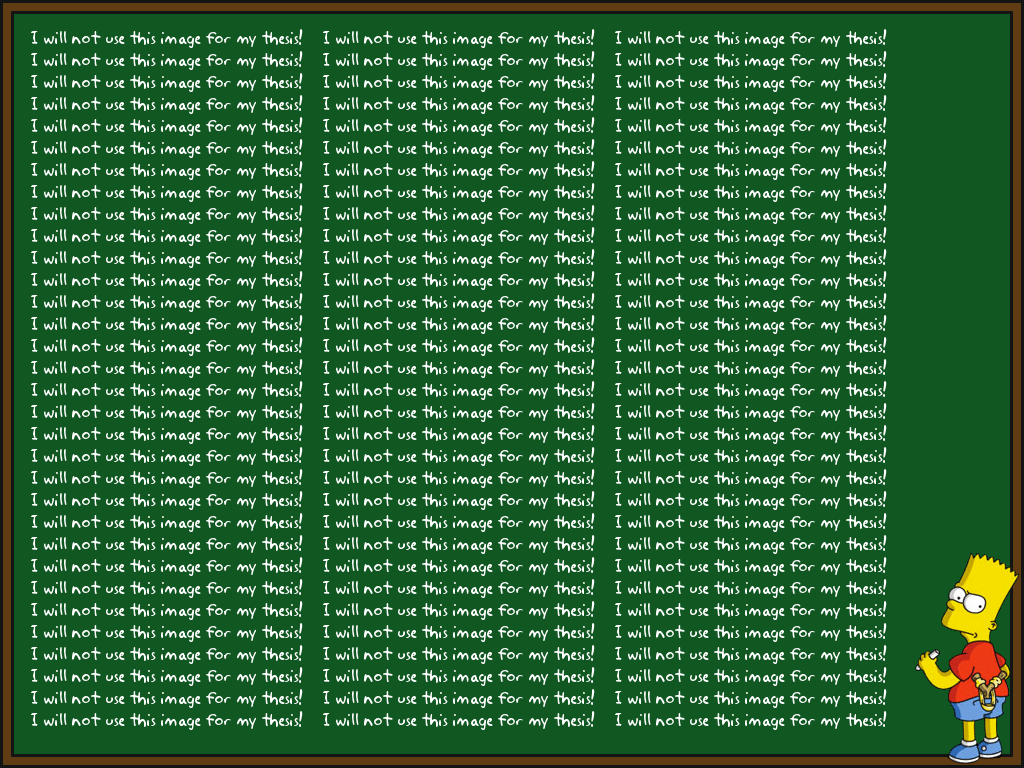
\includegraphics[width=1.0\textwidth]{graphics/not-the-final-title}}

\begin{document}
\selectlanguage{english}
\pagenumbering{roman}
%% titlepage.tex
%%

% coordinates for the bg shape on the titlepage
\newcommand{\diameter}{20}
\newcommand{\xone}{-25}
\newcommand{\xtwo}{150}
\newcommand{\yone}{25}
\newcommand{\ytwo}{-243}

\begin{titlepage}
% bg shape
\begin{tikzpicture}[overlay]
\draw[color=gray]  
 		 (\xone mm, \yone mm)
  -- (\xtwo mm, \yone mm)
 arc (90:0:\diameter pt) 
  -- (\xtwo mm + \diameter pt , \ytwo mm) 
	-- (\xone mm + \diameter pt , \ytwo mm)
 arc (270:180:\diameter pt)
	-- (\xone mm, \yone mm);
\end{tikzpicture}
  \begin{textblock}{10}[0,0](3.35,2.55)
	  \iflanguage{english}  {
\includegraphics[width=.3\textwidth]{graphics/kitlogo_en_rgb}}
                          {
\includegraphics[width=.3\textwidth]{graphics/kitlogo_de_rgb}}
  \end{textblock}
	\changefont{phv}{m}{n}	% helvetica	
	\vspace*{2.5cm}
	\begin{center}
		\Huge{\headtitle}
		\vspace*{2cm}\\
		\Large{
			\iflanguage{english}{Internship report of}			
												  {Diplomarbeit\\von}
		}\\
		\vspace*{1cm}
		\huge{\myname}\\
		\vspace*{1cm}
		\Large{
			\department\\ \institute\\ \iflanguage{english}{and}{und}\\ \fziname
		}
	\end{center}
	\vspace*{1.5cm}
\Large{
\begin{center}
\begin{tabular}[ht]{l c l}
  \iflanguage{english}{Reviewer}{Erstgutachter}: & \hfill  & \reviewerone\\
  \iflanguage{english}{Second reviewer}{Zweitgutachter}: & \hfill  & \reviewertwo\\
  \iflanguage{english}{Advisor}{Betreuender Mitarbeiter}: & \hfill  & \advisor\\
  % \iflanguage{english}{Second advisor}{Zweiter betreuender Mitarbeiter}: & \hfill  & \advisortwo\\
\end{tabular}
\end{center}
}


\vspace{2cm}
\begin{center}
\large{\iflanguage{english}{Research Period}{Bearbeitungszeit}: \timestart \hspace*{0.25cm} -- \hspace*{0.25cm} \timeend}
\end{center}


\begin{textblock}{10}[0,0](4,16.8)
\tiny{ 
	\iflanguage{english}
		{KIT -- University of the State of Baden-Wuerttemberg and National Research Center of the Helmholtz Association}
		{KIT -- Universität des Landes Baden-Württemberg und nationales Forschungszentrum in der Helmholtz-Gemeinschaft}
}
\end{textblock}

\begin{textblock}{10}[0,0](14,16.75)
\large{
	\textbf{www.kit.edu} 
}
\end{textblock}

\end{titlepage}

\pagestyle{empty}
\begingroup
\changefont{phv}{m}{n}
\renewcommand{\baselinestretch}{1}

\begin{titlepage}
  \parindent 0em 
  \LARGE\textbf{\floatingtitle}
  \vspace{24pt}\\
  \iflanguage{english}{by}{von}\\
  \myname \\[1.5cm]
  \begin{center}
  \titlefig\\[1cm]
  \end{center}
  \vfill
  \begin{minipage}{0.4\textwidth}
    \begin{flushleft} \large
      \LARGE\textbf{\thesistype}\\
      \LARGE\releasemonth
    \end{flushleft}
  \end{minipage}
  \begin{minipage}{0.6\textwidth}
    \begin{flushright}
      
\includegraphics[width=1.5cm]{graphics/FZI-Logo}
    \end{flushright}
  \end{minipage}
  \newpage
  \small \thesistype, FZI\\
  \department, \releaseyear\\
  Reviewers: \reviewerone, \reviewertwo
  \vfill
  \fzidepartment\\
  \fziname
  \newpage
\end{titlepage}

\endgroup

% \thispagestyle{empty}

\begin{center}
  \vspace*{\stretch{1}}
  \bfseries
  \LARGE
  \headtitle\\[0.45cm]
  \vfill
  \mdseries
  \huge
  \thesistype\\[0.8cm]
  \large
  Abteilung Technisch Kognitive Assistenzsysteme\\[0.1cm]
  Forschungszentrum Informatik\\[0.1cm]
  an der\\[0.1cm]
  Universität Karlsruhe (TH)\\
  \vfill
  von\\[0.3cm]
  \LARGE
  \myname\\
  \vfill
  \normalsize
  \begin{tabular}{p{3.5cm} p{0.4cm} p{5.5cm}}
    \textbf{Tag der Ausgabe} & : &  \timestart\\
    \textbf{Tag der Abgabe}  & : &  \closingdate\\
    & & \\
    & & \\
    & & \\
    \textbf{Betreuer} & : & \advisor \\
    \textbf{Referent} & : & Prof.~Dr.--Ing.~J.~M.~Zöllner \\
    \textbf{Koreferent} & : & Prof.~Dr.--Ing.~R.~Dillmann
  \end{tabular}
\end{center}

\parindent 1em
\affirmation

Ich versichere wahrheitsgemäß, die Arbeit selbstständig angefertigt, alle benutzten Hilfsmittel vollständig und genau angegeben und alles kenntlich gemacht zu haben, was aus Arbeiten anderer unverändert oder mit Abänderungen entnommen wurde.

\vspace{2cm}
\begin{flushright}\noindent
    Karlsruhe,\hfill {\it \myname}\\
    \releasemonth \hfill { }
\end{flushright}
% \preface

Diese \LaTeX{}-Vorlage, basierend auf \emph{KOMA}-Script-Klasse\index{KOMA-Script} scrbook\index{scrbook}, wurde erstellt, um Veröffentlichungen im Universitätsverlag\index{Universitätsverlag} Karlsruhe in einem einheitlichen Layout zu ermöglichen. Die Dokumentklasse\index{Dokumentklasse} \emph{UVKABook}\index{UVKABook} soll dabei unverändert bleiben. Sollten zusätzliche Pakete geladen werden, muss sichergestellt sein, dass keine Veränderungen am bestehenden Layout erfolgen. Der Inhalt des Manuskripts wird im Unterordner \emph{content} abgelegt und in das Hauptdokument \emph{book.tex} eingebunden. Bestehende Abschnitte etwa für das Vorwort\index{Vorwort} oder die Danksagung\index{Danksagung} können einkommentiert werden. Unter Umständen kann es notwendig sein, dass einzelne Pakete nachinstalliert werden (beispielweise das \emph{KOMA-Script} oder \emph{natbib}\index{natbib}). Das Literaturverzeichnis\index{Literaturverzeichnis} verwendet \emph{bibtex}. Bei Rückfragen wenden Sie sich bitte an den Universitätsverlag Karlsruhe.

\vspace{1cm}
\begin{flushright}\noindent
    Karlsruhe,\hfill {\it \myname}\\
    \releasemonth \hfill { }
\end{flushright}
% 
\abstract

Agnisim ad te diamcon sectet, voloborper aciduis nonsequamet, sequisciduis nonum irilit ea feugait, sequat vero er ip exero odipit lobore magnit nos nibh ex esed exerciduisi tat. Consed et  inci tet aci et atem in ut velenim vent ullum exeril ut laore molorpe riliscidunt la con ulputat ad digna feum quismolesto dolortisl ea feuguercil delit praessim ver ad tem ipit, velit, conse
enis nonsed mod tincipit augue veniametuer aut vulput nonsed molesse miniatuercin hendit in henibh etumsan velessi.
It verilluptat adiatie vel ullum il dolorem zzriuscing et pratinit wis acilismodit adions ad magna autat ulput adip eum do eu faci tem ver ipis at augue ming erit wiscillan hent iliquisl ullam ecte delent ent adiam zzrit aliqui tie volorem inibh essequip enis nullaore vent ametum vullam, velese vullametue verit, sit ex er il ute dolortio commy nos el utat. 
Nons dolore voloborper sed magnit enisisi. Onsenit digna facip ex eraestin ulla consequatie do cons nulla feugiat. Bor irilla feuguer cipsum er autpat. Duis ad minciliquat. Er sis autat ut wis dolorper adion hendre ver sequate molore etuerci exeros nonulla consectet lorpera essequiscip ectet, suscil el utpat luptatum velis nulla...
% 
\ack

Die vorliegende Arbeit entstand während meiner Tätigkeit als wissenschaftlicher Mitarbeiter am Institut für Formalerschließung und Regelwerkskunde der Universität Karlsruhe (TH). Herrn Prof. Dr.-Ing. habil. A. Mustermann danke ich besonders für die Anregung zu dieser Arbeit, die wissenschaftliche Förderung, die stets vorhandene Diskussionsbereitschaft und für die Übernahme des Hauptreferates.

Für die freundliche Übernahme des Korreferates gebührt mein ganz besonderer Dank Herrn Prof. Dr.-Ing. B. Musterfrau vom Institut für Formalerschließung und Regelwerkskunde. Dem Vorsitzenden des Prüfungsausschusses, Herrn Prof. Dr.-Ing. C. Mustermann gilt ebenfalls mein Dank für die kritische Durchsicht des Manuskriptes. Meinen Eltern, die mir durch ihre Redlichkeit und Strebsamkeit immer Vorbild waren, die mir Heimat und Geborgenheit aber auch Freiheit und Interesse für Neues gaben, danke ich von tiefstem Herzen, ebenso gilt der Dank meinen Geschwistern. Für die Geduld und Entbehrungen, die meine Frau Berta und mein Sohn Anton während der letzten Monate aufbrachten und für ihre unendliche Motivation und ihr Verständnis, das sie mir entgegenbrachten, danke ich zutiefst.

\vspace{1cm}
\begin{flushright}\noindent
    Karlsruhe,\hfill {\it \myname}\\
    \releasemonth \hfill { }
\end{flushright}

\begingroup
\changefont{phv}{m}{n}
\tableofcontents
\endgroup

\mainmatter
\renewcommand{\chapterpagestyle}{plain}
\pagestyle{scrheadings}
\pagenumbering{arabic}

\chapter{Introduction}
\section{Motivation}

Imagine you were sitting in your office, dozing off, ready to sleep. As soon as you fell asleep, someone pulled a prank on you and took you to a different room. Shortly afterwards you woke up confused not knowing where you are. What would you do in this situation? You would probably look around to check if you are still inside the building. Then you would try to pinpoint your location based on what you see inside the room. If that was not enough information you could go outside and start exploring the environment. If you have been here before, you would probably be able to recognize some similarities and find out where you are. Then you could just go back to your office, and continue where you left off. It might seem to be an intuitive task for you, however robots cannot solve it quite as easily.

\section{Objectives}

In this work we would like to tackle the kidnapping problem on robots. The first step is to detect whether a kidnapping situation occurred and the second step is to relocalize itself. Detection can be done by determining whether some information from the sensors is missing or whether the perceived environment does not match with the expected one. Recovery can be done by exploring the surroundings while gathering  information of it. If any known features are found, they will be matched with the robot's database. Successful matching means that the robot can use the results to estimate its position in the environment. Otherwise, the exploration continues.

\chapter{Fundamentals}
\section{ROS}
\section{MCA}
\section{Kinect}
\section{Laser Scanner}
3D laser scanner use narrow laser-beam to scan their environment and allow almost continuous scanning - regardless of whether objects are moving or not. As a result, 3D laser scanner gets a set of points which represent the direction and distance of objects in around. Sick LMS100 (shown in Figure \ref{Laser}) has the scanning angle of  270$^\circ$ and has high detection capability.

We can get the output from laser scanner in ROS with sensor\_masgs/LaserScan message. The message is made up of several parts, including header, ranges, and other information of laser scaner. The start and end angle of the scan, angular distance between measurements, time between measurements, minimum and minimum range value are stored in this message. Most important information we need is the angle of each hit and its distance (range) from the scanner.

\begin{figure}[thpb]
      \centering
      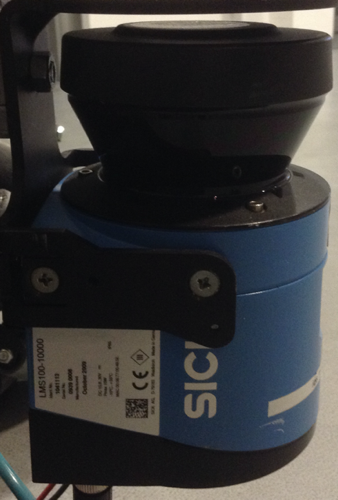
\includegraphics[width=0.5\textwidth]{graphics/Laserscanner.png}
      %\includegraphics[scale=1.0]{figurefile}
      \caption{Sick LMS100}
      \label{Laser}
   \end{figure}
\section{ASAP (Advanced Shared Autonomy Platform)}
The ASAP (shown in Figure \ref{ASAP}), short for Advanced Shared Autonomy Platform, is a mobile robotic platform based on two Segway RMP-50 Omni platforms. The Platform is mounted with four omnidirectional plastic rollers, so that the Segway can free move in all directions (shown in Figure \ref{Omni}). In addition, this ASAP includes some sensors, on-board comoputer, software system. For sensor, there are Two Sick LMS100 laser scanners and a Kinect on top. The embeded computer is Esperia, which has 4G ram, 64G SSD, core i7 M620 CPU and can be connected through WLAN address 141.21.13.215. Ubuntu 14.04 Trusty, ROS Indigo, MCA2 are three main software systems in this ASAP.

\begin{figure}[thpb]
      \centering
      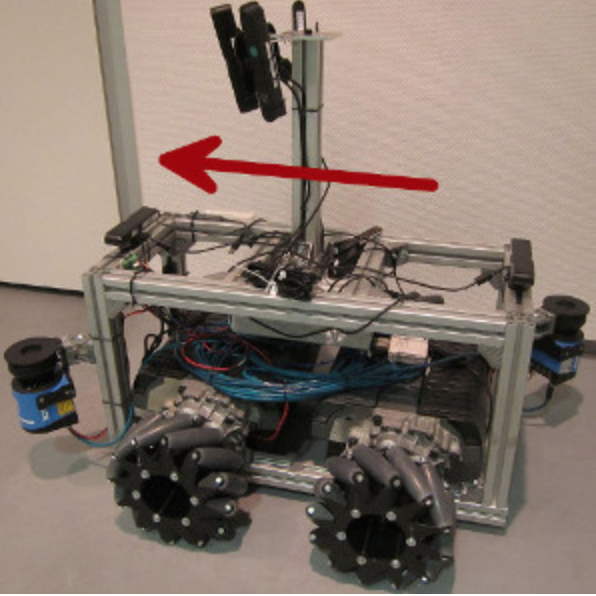
\includegraphics[width=0.5\textwidth]{graphics/ASAP.png}
      %\includegraphics[scale=1.0]{figurefile}
      \caption{The structer of Advanced Shared Autonomy Platform, and red arrow shows the forward direction of the platform, which is the same as the X axes in ROS.}
      \label{ASAP}
   \end{figure}

\begin{figure}[thpb]
      \centering
      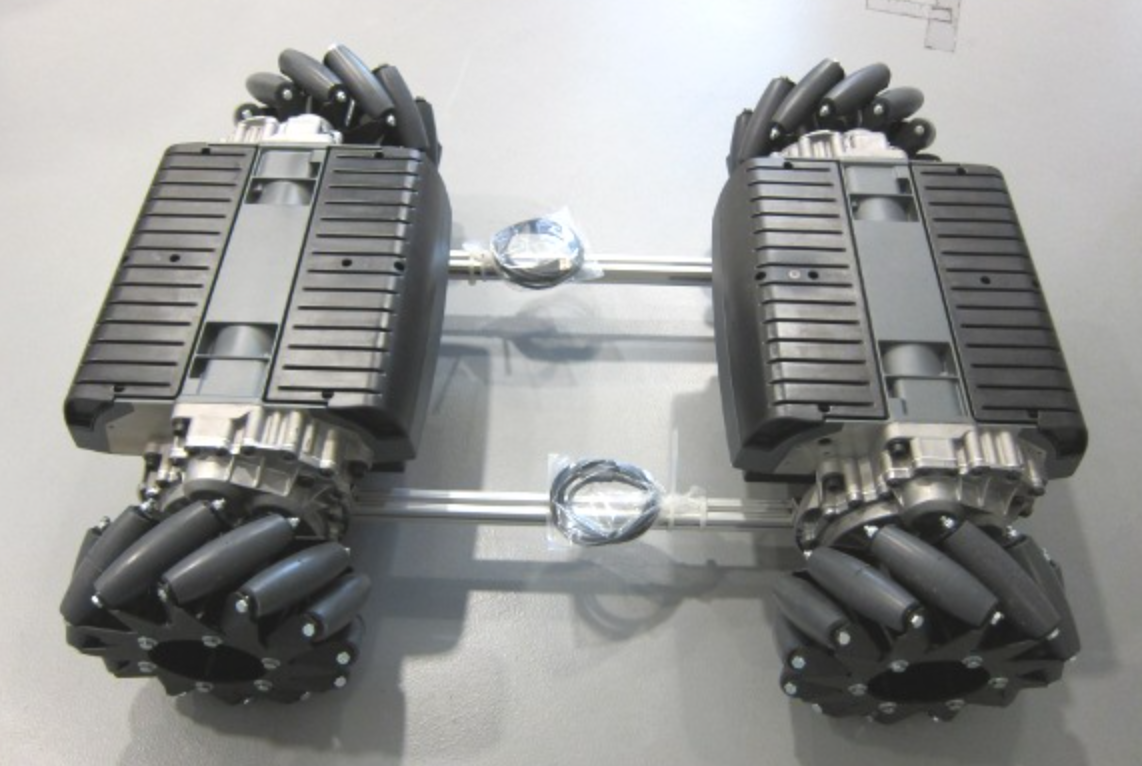
\includegraphics[width=0.5\textwidth]{graphics/SegwayPlattform.png}
      %\includegraphics[scale=1.0]{figurefile}
      \caption{The Segway RMP-50 Omni Plattform includes Mecanum-Rad and Batterie.}
      \label{Omni}
   \end{figure}

\section{Kalman Filter}
Many problems in the domain of artificial intelligence require the prediction of future states by evaluating measurements. Around the 1960s Peter Swerling, Rudolf E. Kálmán, Thorvald N. Thiele and Richard Bucy described an algorithm for this purpose. It is now known as the \textit{Kalman filter}.

In the field of robotics Kalman filters can be utilized to predict future poses for a moving robot by continuously combining measurements from various sources. A Kalman filter is therefore a sensor fusion algorithm. Common sensors are
 
\begin{itemize}
\item motion sensors that estimate position change over time (odometry),
\item laser scanners that scan the environment,
\item cameras that track predefined markers. 
\end{itemize}

By combining the last estimation and the current sensor outputs a new estimation for the current state is obtained. In this process two steps are commonly distinguished: \textit{predict (a priori)} and \textit{update (a posteriori)}.
\\\\
During \textbf{prediction} the next state as well as its covariance are estimated. After that new sensor data is compared with the predicted state, which results in the calculation of the so-called  Gain. The Kalman Gain is an indicator for the certainty of both measurements and prediction. High covariances in the prediction increase the Gain while high covariances in the measurements decrease it.

$$\text{a priori state estimate:} $$
$$\text{a priori covariance estimate:} $$

This will result in the filter trusting either the measurements or the predictions more depending on the gain. 
\\\\
Based on the Gain the Kalman filter produces a posteriori state and covariance estimates during \textbf{update phase}. The higher the gain, the closer these estimates will be to the measurement output and vice versa.

$$\text{a posteriori state estimate:} $$
$$\text{a posteriori covariance estimate:} $$

\chapter{Vision}
The Vision module is responsible for controlling the camera and to publish estimated positions based on seen AR markers. It also notifies the system about any unexpected markers.

\label{Vision chapter}
\section{Working Process}
\subsection{Overview}

We began our project by becoming familiar with ROS, going through  several tutorials on it and setting everything up. In the second step we studied the Kinect along with its functions and possible applications. Next we started integrating \texttt{ar\_track\_alvar} -- AR tag tracking library -- into our project, implemented marker recognition and tracking.Figure \ref{AR tags} shows example tags. Finally we tested the behavior intensively. \\
\begin{figure}
\begin{center}

\includegraphics[width=\linewidth]{graphics/markers.png}
\caption{AR tags}
\label{AR tags}
\end{center}
\end{figure}
In an effort to find the optimal conditions for marker recognition, we tested bundled markers as well as single markers per location (we were limited by the size of an A4 page).

The Kinect's field of view is relevant for this as well, so we determined the maximum possible distance and angle for marker recognition. After generating markers and ensuring their correct and reliable detection, we started working on receiving transform information from \texttt{ar\_track\_alvar} and learned how to interpret it in ROS. We derived world coordinates from it according to the coordinates of the robot and calculated covariances for them.

Afterwards we put our hands on the \textit{Pan-Tilt Unit (PTU),} a device used for head movement. PTU drivers needed to be installed on the computer and its settings were configured. We became accustomed to the basics of PTU movement and designed an efficient algorithm to let the head continuously follow a seen marker, in doing so maximizing the time the robot is in contact with markers.

In the final step we implemented logic for publishing the next expected marker based on the current estimated position. All required markers were generated and placed on walls with fixed distance from each other and simple database including all markers along with their position was built.

During testing we encountered various expected and unexpected problems as well as bugs. We spent a significant amount of time resolving them and finding an appropriate solution for each problem. Although some of them consumed a lot of time to solve, they mostly helped us acquire new knowledge.

\subsection{Tasks assignment}

Starting from October we worked hard to achieve our goals. Our team was formed out of three people, Valeriy Gatuzov, Codrin Goia and Guilherme Pires. Guilherme has returned to his home country at the time of writing, he made his contribution to the documentation separately by writing in the project wiki, so his work will only be briefly discussed here. From the beginning we divided all incoming tasks equally in the group, so that everyone could make a good contribution to the project. Below we outlay the differentiation of tasks in the group:

Guilherme brought extensive knowledge and experience in Linux systems with him, the remaining two of us needed to learn it at first. As we started working on \texttt{ar\_track\_alvar}, Guilherme and Valeriy integrated it into the ROS environment and set it up. At the same time Codrin worked on the data processing from \texttt{ar\_track\_alvar}. He learned a lot about TF-Trees and \texttt{ar\_track\_alvar} itself. Later on he developed an algorithm for transforming local coordinates from markers sent by \texttt{ar\_track\_alvar} to world coordinates and to publish them to the other groups.

Meanwhile Valeriy calibrated marker recognition, generated markers and worked himself through all sorts of errors delegated to him from other teammates. Later on Guilherme implemented an algorithm for computation of the covariance. Valeriy started working on tracking markers with the Pan-Tilt Unit and was challenged with problems like finding an appropriate mathematical function to implement the movement, calibrating the turning speed, stopping the head on time, and at testing and debugging it.

Almost at the end we worked on the next expected marker problem, discussed the details and all possible solutions, then made a concept algorithm, that was implemented by Guilherme and Codrin. Then Valeriy  tested the entire software, writing a testing program and resolving new-found errors. Codrin concentrated on an unexpectedly appeared problem concerning the computation of coordinates which he successfully fixed.  

\subsection{Used Resources} 

We used a lot of open source resources, that were essential to our success. From the beginning we learned a lot about Linux, because we did not have much experience in it. Then we became familiar with ROS, its packages, nodes, core commands and its functioning principle in general. We learned all the concepts starting from catkin and roscore, all the way up to tf. As a visualizalation and debugging tool rviz was very helpful for verifying e.g. if axes direction are correct. rqt\_graph helped us understand the connection between different nodes. We successfully employed the Kinect in our work for recognition of markers which were generated with \texttt{ar\_track \_alvar} -- an open source AR tag tracking library for ROS. We used ``createMarker'' -- another useful tool and part of \texttt{ar\_track\_alvar}, that helped us create a graphical representation for bundles of markers as well as for single markers. Each time it generates an XML file for it. Later on, when we started working with Pan-Tilt Unit for the purpose of moving the head, we installed \texttt{flir\_ptu\_driver}, \texttt{ptu46} and \texttt{ptu\_control} in order to be able to control the PTU.

\section{Conceptual Design}

\subsection{Components}
At a conceptual level, the Vision package can be decomposed in two components, implemented in two ROS nodes: \texttt{localizer} and \texttt{marker\_broadcaster}. The internal interaction between them and all other external nodes does not need to be understood or changed from the exterior, as the whole setup is launched in the custom \texttt{vision.launch} file of the package Vision.
The \texttt{marker\_broadcaster} node is responsible for feeding the tf system with the position of all markers inside the database. \texttt{localizer}, being the node containing the main functionality, deals with the processing of data from the Kinect camera and uses the tf data from \texttt{marker\_broadcaster} in order to output a position with covariance. Figure \ref{Vision Concept} shows how the data flow inside the Vision package undergoes several transformations in order to output the position of the camera:

\begin{figure}[h]
\begin{center}
\includegraphics[width = \linewidth]{graphics/vision_concept.png}
\caption{Transformations from input to outpout}
\label{Vision Concept}
\end{center}
\end{figure}

Since the navigation will only take place in one plane which the robot will never leave, all the 3D data is filtered out as soon as possible to keep computations at the appropriate level and to avoid computation of unnecessary data. This takes place immediately after the interpretation of marker position coming from \texttt{ar\_track\_alvar}. From that point on coordinates in the whole system will only have 3 values, namely x coordinate, y coordinate, and rotation around z-axis. 

\subsection{Dependencies}
The main purpose of the Vision group is to collect data coming from the Kinect camera, process it and output a data in form of a position on the map. Secondary purposes are the signalization of a seen marker, signalization of an unexpected marker, as well as commands to the Pan-Tilt Unit rotation in order to rotate the head towards the seen or expected marker. In other words, the role that the vision package plays is to serve as a mediator between external ROS nodes feeding it with raw data and generating useful data for the Kalman and High Level Components to process. In order to be able to work, all external dependencies need to be present when being launched. At a conceptual level, these dependencies are:

\begin{enumerate}
\item External ROS packages publishing from outside the project:
\begin{itemize}
\item \texttt{freenect\_launch} for collecting data from the Kinect camera
\item \texttt{ar\_track\_alvar} for processing image data from \texttt{freenect\_launch} and output marker positions
\item \texttt{flir\_ptu\_driver} for managing camera rotation
\end{itemize}
\item Internal ROS packages publishing from inside the project: 
\begin{itemize}
\item High Level
\item Kalman
\end{itemize}
\item Marker positions database in form of a text file.
\end{enumerate}

\subsection{Interactions with other Groups}
Information between the Vision package and the other components of the project is done using the standard ROS messages. The main node from the Vision package publishes pose information coming from higher level nodes of Kalman and High Level group and subscribes to the incoming processed data coming from them.

\begin{description}
\item Output topics:
\begin{itemize}
\item vision/estimated\_pose topic: main topic, in which the position of the robot with respect to world coordinates is published
\item vision/sees\_marker topic: is publishing only when a marker has been seen. 
\item vision/unexpected\_marker  topic: it is intended to serve as a trigger to High Level group in order to signalize that a kidnapping might have occurred.
\end{itemize}
\item Input topics:
\begin{itemize}
\item HL/is\_kidnapped topic: In case of a kidnapping, the camera rotation enters a searching state, where it is constantly spinning in search of a new marker.
\item kalman/fused\_pose topic: represents the final estimate of the robot position and is used in the computation of the next expected marker in case no kidnapping situation is active. By knowing the estimated position, the location of the nearest marker can be computed and in case nothing is seen, the camera rotates towards that direction.
\end{itemize}
\end{description}

\section{Implementation}

\subsection{Input/Output Specification}
The Vision package communicates with other ROS nodes exclusively through topics. There are input and output ports, local topics that stay within the project to communicate with other teams, and global topics that go outside the project to reach for data input and to send commands.

\begin{itemize}
\item geometry\_msgs::PoseWithCovarianceStamped: output internally to topic ``vision/estimated\_pose''. Represents the main functionality of the vision package, i.e. to provide global robot coordinates computed from camera input and marker database.
\item std\_msgs::Bool: output internally to topic ``vision/sees\_marker''. Is publishing true whenever a marker is identified by the Kinect camera.
\item std\_msgs::Bool: output internally to topic ``vision/unexpected\_marker''. Is publishing whenever the position it receives from Kalman group does not match with the currently seen marker
\item std\_msgs::Bool: input internally from topic ``HL/is\_kidnapped''. Used to decide the camera rotation strategy: whether it shall rotate in search of a marker, or rotate towards expected marker on the map.
\item geometry\_msgs::PoseWithCovarianceStamped: input internally from topic ``kalman/fused\_pose''. Used to determine the distance, direction and finally the ID of the next expected maker.
\item ar\_track\_alvar\_msgs::AlvarMarkers: external input from topic ``ar\_pose\_marker''. Receives seen marker ID and transform in camera coordinates.
\item sensor\_msgs::JointState: external input from topic ``joint\_states''. Used to read the current angle between camera and robot.
\item sensor\_msgs::JointState: output externally to topic ``ptu/cmd''. Used to pass commands to the PTU unit when rotating toward next expected marker or when tracking the currently seen marker.
\end{itemize}

\subsection{Class Dependencies}
In order to collect the image data coming from the Kinect, process it and output a position with covariance, several classes of the ROS library are used. A diagram showing all dependencies can be seen below in figure \ref{Vision Dependencies}.

\begin{figure}
\begin{center}
\includegraphics[scale = 0.8]{graphics/vision_dependencies.png}
\caption{Class dependencies inside Vision Package}
\label{Vision Dependencies}
\end{center}
\end{figure}

\subsection{Package Diagram}
Since the Vision package serves as a link between low level input data in form of image stream and output in form of position, it heavily relies on foreign packages for data acquisition and processing as illustrated in figure \ref{Vision Package Diagram}. Note that the arrows indicate the flow of data inside the topics (from publisher to subscriber), that means arrowheads are positioned exactly opposite to dependency relationships.

\begin{figure}
\begin{center}
\includegraphics[scale = 0.6]{graphics/vision_package.png}
\caption{Flow of data between packages}
\label{Vision Package Diagram}
\end{center}
\end{figure}

\subsection{TF Tree}
In order to position the robot correctly in the world, the tf data between all known coordinate systems is put together in order to compute the missing link: the transform of the robot in world coordinate system. The localization process is initiated only when a marker is seen and consists of two stages, each one implemented in its own thread.

First step: When a new marker is seen by \texttt{ar\_track\_alvar}, the transform of the marker with respect to the camera is converted into 2D in order to get rid of unused data. The inverse is then applied on the transform so that it now represents the position of the camera in marker coordinates.

Second step: The transform of the seen marker with respect to world is taken from \texttt{marker\_broadcaster} node providing the missing link to computing the position of camera in world coordinates. However the process is not finished here. Although the robot has the same position as the camera, it does not necessarily have the same rotation, since the angle between robot and camera may vary.

So as a last step, the transform is rotated accordingly (with the negative angle between robot and camera received from \texttt{flir\_ptu\_control}). The result represents the final position of the robot in world coordinates. Figure \ref{TF tree} gives an overview of the transformation tree.

\begin{figure}
\begin{center}
\includegraphics[scale = 0.35]{graphics/vision_tf.png}
\caption{TF tree used during localization computation}
\label{TF tree}
\end{center}
\end{figure}

\subsection{Thread Overview}
A total of 4 threads are active inside the running localizer node, that are communicating via global variables with each other.

\begin{itemize}
\item Thread inside function \texttt{alvarCallback}: This is the most important thread and responsible for acquiring data in form of markers from \texttt{ar\_track\_alvar}. After converting it into 2D, it computes the inverse in order to obtain camera transform with respect to marker, and publishes them to the tf tree. Additionally it computes the next expected marker and in case the next expected marker does not match the currently seen marker, the unexpected marker is signalized to the high level group. An important notice is that the unexpected marker is not published immediately.

The computation of the expected marker is done based on the position, \texttt{fused\_pose}, that the Kalman group is publishes. Due to the fact that this data may contain noise, for some frames the position of the robot may not be signalized correctly, leading to a false positive when signalizing the unexpected marker. For this reason the system does not signalize it until the error persists for a small number of seconds (default is two) until it can safely be stated that the current computed position cannot be explained by the seen marker.

\item Thread inside function \texttt{publishTransforms}: This thread is responsible for extracting the world transform  of the camera from the tf tree, rotate it in order to get robot transform, and publish it to the other groups in the ros topic “vision/estimated\_pose”. The rotation is the only thing that needs to be done to switch from camera transform to robot transform, and is done by knowing the angle between these two components. The angle is provided by another thread listening to data coming from the PTU unit by means of a global variable.

\item Thread inside \texttt{ptu\_thread} function: This thread is responsible for the processing of data related to the PTU unit. It reads the current joint state and has two functioning modes for giving commands to the PTU, based on the visibility of the marker. In the first case, if at the present moment  there is a visible marker, it computes the angle representing the offset of the marker from the center of the camera. Then it gives the command to the PTU to rotate the camera by that angle, so that the camera is always facing the marker, allowing it to track a marker even if the robot is moving.

Given the fact that \texttt{ar\_track\_alvar} is feeding the system with seen marker coordinates in camera reference system, this angle is easy to compute using the \textit{arctan} function. In the second case, which occurs if at the present moment there is no marker visible, the role of the thread becomes to rotate the camera towards the next expected marker.

First of all, the estimated position coming from Kalman group is read. Then, the next expected marker is computed as the nearest marker next to our current estimated position. Finally, by having the transform of the expected marker, as well as our current estimated transform, the tf tree is used to compute the position of the expected marker in robot coordinates. The angle is computed by means of the atan2 function and the command is given to the PTU to rotate accordingly.

\item Thread inside function \texttt{publishTransformFromHL}: This is a tiny thread and simply reads the estimated pose coming from the High Level group and stores them in the global variable \texttt{fused\_pose} so that it is accessible to other threads.
\end{itemize}

The communication between threads by means of global variables is represented in table \ref{Thread Communication} below. For each global variable the threads accessing it are displayed.

\begin{figure}
\begin{center}
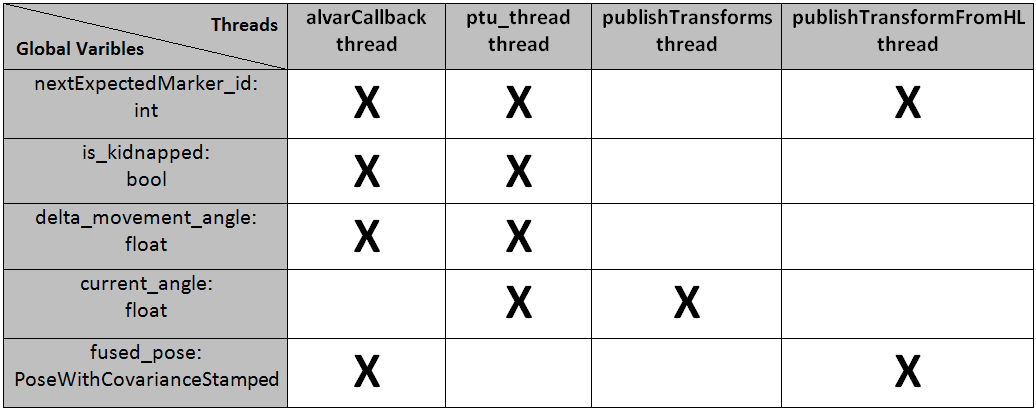
\includegraphics[width = \linewidth]{graphics/vision_threads.png}
\caption{Thread Communication}
\label{Thread Communication}
\end{center}
\end{figure}

\section{Problems and Challenges}

As already mentioned, there were as usually a lot problems practically from the start. But all of them are successfully resolved now and we have learned a lot from them. Here some of the problems we had will be briefly shown.

The first problem that confronted us was incorrect setup of the \texttt{ar\_track\_alvar} launch file, it was not meant to work with \texttt{freenect\_launch}, so we had to change the start connection between nodes, so that \texttt{ar\_track\_alvar} gets data from the Kinect. The next problem occurred when computing the covariance. The values we received from the algorithm were too inaccurate. We solved this problem by finding and implementing a queue with the right size of 25 samples, so the program has enough data in order to give back a usable covariance. After that we spent time thinking about the required size of the marker, so that we could maximize the distance from which Kinect will be able to see a marker. We tried bundles of markers, i.e. two and three markers on one, tried single markers and then settled with this solution since it is good enough for our needs.

Moreover we worked on the problem of positioning markers on the map (i.e. in the building), so that they are not too far away from each other and on the other hand so that there are not needlessly many of them on the map. Otherwise it would be irritating for the robot to see two markers at the same time. That problem was found while implementing an algorithm for the next expected marker.

Then, when working with PTU we had a problem developing the procedure to turn towards the expected marker. $atan$ is not defined at all locations, so at the end we used $atan2$, because it considers all special cases. Afterwards we had a problem with stopping the head when it was already looking in the marker's direction. We solved it by lowering accuracy for marker following. One of the last problems were the axes, that were not parallel to each other. We saw it in rviz and needed to dive into the code once again to find an error. The problem was found in the wrong implementation of the database. After we changed it, everything was working fine. 

\section{Testing}

Our first test was to find out how far the robot can go, while still being able to recognize the marker. We discovered that the viewing angle is approximately 58 degrees and viewing distance is 3.4 meters. Figure \ref{Field of View} visualizes the field of view.

After that we decided to put every marker on the wall within 2,5 meter distance. It turned out to yield good results. Then we worked on PTU movement to determine the optimal speed, so that it will neither turn too slow nor too fast. We came to the conclusion that 0,7 radians per second results in smooth and natural movement. Additionally we wrote a dummy program to verify that all values are interpreted as expected. By the time we ended up testing our software, we were practically done with our part of the project.

\begin{figure}
\begin{center}
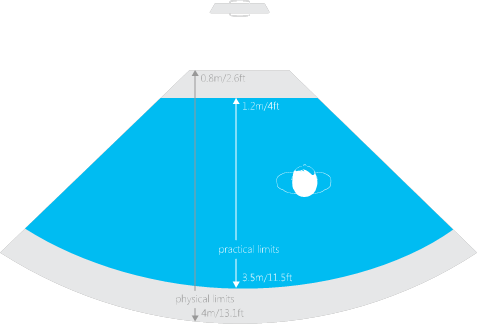
\includegraphics[scale=0.8]{graphics/view_field.png}
\caption{Field of View}
\label{Field of View}
\end{center}
\end{figure}

\chapter{EKF (Extended Kalman Filter)}
\section{ROS Package Dependencies}
\subsection{Robot localization}
For the functionality of the Kalman Filter the package \texttt{robot\_localization} was used. The package provides a convenient 15-dimensional implementation of the kalman filter with direct support for 6D pose, 6D velocity and 3D acceleration vector. The available inputs can be dynamically configured in the \textit{launch file} for the \texttt{robot\_localization} node. In general the whole package is configurable via launch file or yaml file.

\subsection{TF (Transformation)}
The \texttt{TF} package is used to define all sorts of data transformations in different coordinate systems. In this case the robot's map data and the input of the marker detection are converted to be fused in a common coordinate system. 

\section{Package Structure / Design}
\subsection{Configuration}
The Kalman package is highly dynamic. All properties and settings can be configured by yaml files and launch files similar to the \texttt{robot\_localization} package. So no recompilation is required if topic names are changed or the resulting frames of the data change.

\subsection{Robot Localization Node}
This node is a part of the \texttt{robot\_localization} package and implements the Extended Kalman Filter. It receives input from the topics of the Vision module INSERT NAME, the robot's map system and a third topic generated by the Kalman converter node in case the robot is kidnapped to prevent the continuous detection of kidnappings due to jumping output values.

\subsection{Converter Node}
The converter node handles the output of the \texttt{robot\_localization} node and republishes the data to the final topic INSERT NAME, the other modules are working with. This interception is used to filter all results of the robot's map data and only rely on camera data as long as the robot is in kidnapped state.

Moreover in case of a kidnapping the converter node publishes the camera results with reduced covariance as a third input topic to the Kalman Filter, to convince it that the camera data now has the only valid results. This is needed since the ranges of covariances between the different input topics vary vastly.

\section{Testing}
\subsection{Matlab Parameter Simulation}
In the beginning of the project a Matlab simulation of a Kalman Filter was created to experiment with the different parameters of a Kalman Filter and to learn how they influence estimation.

By inserting velocity data and analyzing the predictions we gained much insight into the Kalman model. Additionally the effects of the noise covariances became much clearer in a way that was very helpful throughout the project.

\subsection{Test Data Generation}
In the first months of the project it was very difficult to test the implementation since all teams started from scratch. Production and publication of sensor data was just being developed. To overcome this obstacle artificial test data was generated with two approaches.

\subsubsection{Matlab}
In Matlab test data was generated by supplying a number of points distributed in time and then using a cubic spline interpolation to generate the values in between. For simplicity this values where initially generated only for one dimension of the Kalman Filter.

\subsubsection{Simple MonoGame}
For the generation of more realistic 2D poses and view angle of the robot a small \texttt{C\#}-program was built. This program uses the MonoGame framework to allow mouse interaction on a small window. A small arrow is displayed to represent the robot. Then by clicking on a position the user can tell the robot to move there with a pre-defined fixed speed. When holding down the mouse button and releasing it on another pixel the vector between these points is used to generate the target view angle of the robot. In the background the program continuously writes the current position and view angle of the robot to a file.

\subsection{Sensor Test Data Dummy node}
Next placeholder sensor nodes were written that do nothing but read simulation data from file and publish them in a loop. This way the Kalman Filter could be tested even if the actual sensor nodes were still in development. It was now possible to tweak the many parameters of the \texttt{robot\_localization node} and study the filters behaviour independently of the other groups.

\subsection{Rviz Simulation}
After development of the input and procesing pipeline for test data the next challenge was to evaluate the filter's outputs. Since humans are very ineffective in classifying text data, the ROS package \texttt{rviz} was utilized to visually compare input data and filtered result. The visual proof for the effects of parameter changes greatly enhanced our capability to evaluate the Kalman filter's performance.

\subsection{visualization node}
The visualization node subscribes to the output topic of the Kalman Filter and the input topcis from the robot to create displayable data which can be used to verify the data fusion quality. This displayable data are markers published to \texttt{rviz} that shows them in its coordinate system. There are two possible visualization modes:

\begin{itemize}
\item Show the current 2D Pose of the robot
\item Show timely change of the robot's pose in x.
\end{itemize}

It is also possible to display process covariances over time to gain a better understanding of why there might be a sudden change in the kalman filter's behaviour.

\section{Difficulties}
\subsection{Initial start with custom Kalman Implementation}
Before using the \texttt{robot\_localization} package a quick attempt to implement the Kalman Filter manually was investigated. Luckily our attention was directed towards the \texttt{robot\_localization} package before more than data subscription and publishing were implemented, both of which were fortunately reused throughout the project.

\subsection{Difficulties with employing MCA2}
When the Kalman Filter performed satisfactorily with the artificial test data, the next step consisted of producing more realistic data with a true robot simulator. For this MCA2 appeared to be a suitable solution. But the installation of MCA2 and the simulator presented unexpected difficulties and failed in the end.

One of the reasons is the quality of the MCA2 documentation which posed a major problem. It is highly fragmented, redundant, often outdated and in some places contradictory. Very often it was difficult to understand if an installation error was caused by a user mistake or by the documentation and if the latter, whether it is only unclear, incomplete or incorrect. 

The usual approach for a computer scientist is to read the documentation and rule out any self-made errors before asking possibly unnecessary questions. This is why the lacking documentation caused more harm than good.

It was finally discovered that additional data only existing on a USB drive was required in order for the package to install successfully. But even after having received this piece of data the software could only be run exclusively on lab computers, indicating another still unknown dependency or requirement.

By that time data publishing and necessary software for it have already been facilitated on the robot. So MCA2 was abandoned and the robot itself was used to generate data.

\subsection{Roslaunch initialization and ROS\_IP behind NATs}
While working with virtual machines for ROS package development the problem of incorrect communication between the packages was discovered. Only when starting the nodes in the right order with appropriate delays in between, the system would work on the robot. In general the specification of the \texttt{ROS\_IP} environment variable is used to solve that issue. The local IP of the virtual machines behind a NAT was not available and so the execution of the nodes was completely moved to the robot.

\subsection{Wifi Overload $\Rightarrow$ huge delays}
When attaching the camera to the robot in a manner that the image data has to be sent over wifi, the whole ROS communication is extremly slow. This problem is solved by installing all drivers for the camera on the robot. So the camera and its related nodes can operate locally on the robot.

\subsection{Boundary for accepted jumps between sensor outputs}
When first configuring the \texttt{robot\_localization} package, a threshold for tolerated jumps in the sensor data was set to a rather low value. This caused the Kalman Filter to exhibit a lot of unexpected behavior, for instance it did not respect changes in one sensor at all. After setting the threshold to an appropriate value, the filter worked even better as initially expected. This is partly due to the well adjusted remaining parameters of the Kalman Filter which were already thoroughly tested with the Matlab simulation.

\subsection{Set pose of robot\_localization does not work as expected}
The \texttt{robot\_localization} package provides a \texttt{set\_pose} topic to force the actual pose of the robot. It was planned to use this topic to inform the Kalman Filter about the new pose after having recovered the robot from kidnapped state. Unfortunately this sets the pose permanently and further input is ignored, so another solution was necessary. The final approach uses a third virtual input sensor that sends the recovered pose along with very low covariances to convince the Kalman Filter to trust this source the most.

\subsection{Unclear information about the data source topics and types for the data fusion}
Finding out which scripts must be started on the robot to make it publish its pose and twist turned out to be a challenge in itself. During some periods alternative topics were used to at least receive any data to work with. For example the map position of the robot was temporarily replaced by its odometry output.
\chapter{High Level}
\section{Overview}
\section{Implementation}
\subsection{Detection}
\subsection{Recovery}
\section{Problems and Difficulties}
\subsection{Calibration}
\subsection{Floor Level}
\subsection{Uneven Surface}
\subsection{Transparent Window}
\chapter{Evaluation}
\section{Integration}
Due to the consequent usage of IDSGit as version control tool, the development process can be reviewed in the git commit history. Merging the groups' development branches was quite simple and required only minor fixes, primarily to correct hard-coded file paths or to add missing files to the repository. Additionally, of course each group's dependencies needed to be installed.

After all modules compiled together successfully, the actual integration work started. The main integration work consisted in correctly delivering and receiving data between the groups, to make the modules act together as expected. For instance all subscribed and published topics required adjustments to match the requirements discussed in advance. Aside from that some topic names had to be updated since every group used their own topic namespace. The main part of missing specification turned out to be the frames each group publishes their data in.

One unanticipated problem arose when deploying the camera on the robot: Testing the camera related code with the Kinect attached to the robot caused high wifi latency. Since all nodes still operated on development machines, image data from the camera kept being sent uncompressed over the network and massively slowed down all work. So help from authorized users was needed to install drivers for the camera on the robot. From then on the Vision nodes operated directly on the robot.

\section{Test Scenarios}
The implementation was tested in three scenarios with increasing difficulty levels. Evaluation of the robot's behavior was done by comparing expected reactions with actual behavior, by visualizing sensor outputs in rviz and by reading out the ``is\_kidnapped'' topic. The scenario rules and results are presented in the following.

\begin{description}
\item[1. Marker tracking] Localization with laser scanners is disabled and the robot is moved while its camera is in contact with a marker. No actual kidnapping takes place, this only ensures that the robot moves its head correctly to stay in contact with the marker.

The scenario was handled correctly by the robot. First it scanned the entire room rotating the camera by a full 360$^\circ$. After that the camera was focused on the found marker. We noticed small jerks to the left and right though, which probably is a result of too big single rotation steps that keeps causing the robot to believe that it needs to make a small correcting rotation back to the other direction.

\item[2. Trivial kidnapping] Both laser scanners and camera tracking are disabled before kidnapping the robot. At the new location the camera is in immediate contact with a marker. This was done by turning off laser scanners and odometry, covering the camera with a cloth and placing the robot in front of a marker.

Recovery from kidnapped state took place immediately after lifting the cloth. The marker was focused just like in scenario 1 and the rviz visualization showed the correct position.

\item[3. Real Kidnapping] Finally the robot is kidnapped like in scenario 2 but is not provided with a marker. For this we again placed a cloth on the camera and kept it there longer and hiding surrounding markers in doing so. That way exploration was prolonged and could be tested more extensively. 

The robot first turned around on the spot to scan its surroundings while rotating the camera. After it found the closest obstacle (a wall), it positioned itself left from it and kept moving in one direction according to the maze-solving-algorithm. Simultaneously, it kept rotating the camera to search for markers. The wall ended in a pillar where the cloth was lifted to reveal the camera. The robot performed a successful u-turn and found the marker on the other side of the wall.

This test scenario revealed the difficulties of navigation on uneven paths. The location around the pillar was very uneven so that the robot needed several attempts in which it also temporarily moved backwards to turn there.
\end{description}

\chapter{Conclusion}
\section{Summary and Conclusion}
The kidnapped robot problem can be solved effectively with a robot featuring a Kinect, laser sensors and odometry data.

In this project marker tracking and camera-derived position estimates were generated. A database for markers was built and logic for determining the next expected marker was implemented. Various sensor outputs were merged and filtered by an extended Kalman Filter, the filter behavior was adjusted to be able to cope with varying data quality and different numbers of sensor sources. Conversions between various frames were established. Decision making based on available position data was implemented. A maze-solving-algorithm was employed for map exploration. Contradicting information from sensors as well as high covariances in position estimates were used to determine kidnapping situations. Rviz was heavily used to debug and monitor the software.

Separating the problem into data acquisition task, data processing task and logic task, then solving it in three autonomous groups is easy and saves time. Occasional meetings are enough to discuss the strategy and to define communication interfaces. This approach requires the generation of dummy test data to serve as placeholders for other groups' outputs. It saves tremendous time to document all learned rules and usages for institute specific tools (be it hardware or software) in a shared wiki so that all teams can benefit from it.

\section{Outlook}
In the future the next obvious step is to explore the possibility and requirements for camera tracking of natural markers instead of AR tags. Although AR tags are easy to use and quickly setup, they cannot be attached to arbitrary surfaces, either because of practical or simply because of optical reasons. Related to this, a marker database for the entire FZI might be very interesting for more elaborate tests and use cases.

Additional sensors can be added to further improve localization accuracy and allowing the robot to recover from more complex kidnapping scenarios.

In the long run it will be necessary to smoothly integrate kidnapping recovery as a background service on robots. At the moment the camera keeps tracking markers as soon as they are in range, thus rendering it useless for the robot's main task.

\pagestyle{scrplain}
\appendix

\chapter{Analysenmethoden zur Bestimmung der Reaktionsvariablen }

\section{Gaschromatographie}

Die Bestimmung des Wasserstoffanteils mit dem GC HP-5880 A Series erfolgt durch eine Temperaturrampe. Zuerst wird die Temperatur fünf Minuten lang bei $50 ^{\circ}C$ gehalten. Danach wird bis $130 ^{\circ}C$ ($15 ^{\circ}C/min$) aufgeheizt. Der GC besaß eine gepackte Trennsäule (Porapak Q). Als Detektor stand ein Wärmeleitfähigkeitsdetektor (WLD) zu Verfügung. 

Der GC HP 6890 ist mit zwei Säulen ausgestattet, eine für die Bestimmung von Wasserstoff (80/100 Hayesep Q, 2 m lang)  mit Stickstoff als Trägergas, und eine andere Säule (60/80 Molekularsieb, 4 m lang) für CO2, Stickstoff, Sauerstoff und Kohlenwasserstoffe ($< C4$), in der Helium als Trägergas benutzt wird. Für die Konzentrationsmessung wurde zwei Detektoren verwendet: ein Wärmeleitfähigkeitsdetektor (WLD) und ein Flammenionisationsdetektor (FID), die in Serie geschaltet waren. 

In dem WLD wird die Wärmeleitfähigkeit des Trägergases (Stickstoff) mit der der gaschromatographisch getrennten Substanzen verglichen. Der Vergleich erfolgt an einer Wheatstoneschen Brücken. Solange nur Trägergas durch die Wheatstoneschen Brücken fließt, wird die Wärme vollständig abgeführt. Wenn andere Substanzen mit geringe Leitfähigkeit in die Messzelle gelangen, entsteht ein Wärmestau am Hitzdraht (Platin), der den elektrischen Wiederstand erhöht. 

Für die anderen Komponenten in der Gasphase wird ein FID benutzt, der für Verbindungen mit C-H oder C-C Bindungen eine deutlich höhere Empfindlichkeit besitzt. Die Verbrennung der Komponenten läuft über die Bildung von Radikalen, durch die die Ionisation erhöht wird. 

Die Messung erfolgt während 31 Minuten. Die Temperatur wird von $60 ^{\circ}C$ auf $220 ^{\circ}C$ erhöht. Zuerst wird nach der Probeeinspritzung die Temperatur bei $60 ^{\circ}C$ zwei Minuten lang gehalten. Dann erfolgt eine Aufheizungsrate von $5 ^{\circ}C/min$  bis eine Temperatur von $160 ^{\circ}C$ erreicht wird. Anschließend steigt die Temperatur bis $220 ^{\circ}C$ mit einer Aufheizungsrate von $15 ^{\circ}C/min$. Bei $220 ^{\circ}C$ wird die Temperatur während  5 min konstant gehalten. 

Die Gasproben werden mit Gasspritzen aus zwei Probenehmern  gezogen.  Ein erster Probenehmer befand sich direkt an der Stelle der Phasentrennung, der zweite war hinter dem Abwasserbehälter angebracht. 
Zur Kalibrierung der Gas-Chromatographen wurden täglich Gasproben mit bekannter Zusammensetzung eingespritzt. Da die Gas-Chromatographen von mehreren Arbeitsgruppen bedient wurden, war eine Ausheizung des GC während mehreren Stunden nötig, die jedes zweites Wochenende durchgeführt wurde.  Die Versuchsplanung hängte davon ab, dass die Gasproben gemessen werden konnten.

\section{Analyse zur Bestimmung des Kohlenstoffgehalts im Abwasser}

TOC-Messgerät (DC-190 Rosemount-Dohrman) 

Das Messprinzip besteht aus einer hochtemperatur-katalysierten Verbrennung der Abwasserprobe. Die Verbrennung findet in einem Quarz-Rohr statt, das  gepackt mit dem Katalysator Pt/Al2O3 ist. Die Ofentemperatur  beträgt $800 ^{\circ}C$. Durch die katalysierte unterstützte Oxidierung mit reinem Sauerstoff ($250 ml/min$), werden die Abwasserproben vollständig zu CO2 und Wasser umgewandelt. Das entstehende CO2 wird von dem Wasser in einem Kondensator-Gas-Flüssig-Trennungssystem (Kupfer-Zinn-Adsorber) gereinigt. Die Halogene werden von dem Gasprodukt getrennt. Die reine CO2-Menge wird anhand eines Infrarotdetektors ermittelt. Anorganischer Kohlenstoff (IC) wird mit einem IC  Reaktor bestimmt, der Phosphorsäure 20 \% enthält. In diesem säuerlichen Medium werden die  anorganischen Carbonate der Abwasserprobe zu CO2 umgewandelt. Das entstehende Gas wird zum Trennungssystem geleitet und mit dem Infrarotdetektor gemessen. Die Genauigkeit dieses Messprinzips lag um etwa 2 \%. 

Küvetten-Test LCK 381 (Dr. Lange GmbH, Düsseldorf, D, Messbereich 60-735 mg/l)

Die Proben müssen verdünnt werden, wenn der Messbereich überschritten werden könnte.  Zur Bestimmung des Gesamtkohlenstoff-Gehaltes (TC) wurden $200 \mu l$ der verdünnten Abwasserprobe in die mit dem Aufschlussreagenz (Natriumperoxidsulfat) gefüllte TC-Küvette (KD 381 B) pipettiert. Nach dem Verschließen mit Originaldeckel und mehrmaligem Umschwenken wurde die TC-Küvette mit einer vorbereiteten Indikatorküvette (LCK 380/381) durch einen Membran-Doppel-deckel verbunden. Gleichzeitig wurde die TiC-Küvette (KE 381 B) mit $1 ml$ der Probe befüllt. Analog zur Aufarbeitung der TC-Bestimmung wurde die TiC-Küvette mit dem Originaldeckel verschlossen und mehrfach geschüttelt. Im Anschluß daran wurde die TiC-Küvette mit der entsprechenden Indikatorküvette verbunden. Beide Küvettenkombinationen wurden gleichzeitig in einem vorgeheizten Thermostaten LT 100 (Dr. Lange GmbH) 2 h bei $100^{\circ}C$ erwärmt. Während der Erwärmung reagieren die Abwasserproben mit dem Reagenz und es entsteht CO2, das den Indikator verfärbt. Nach dem Abkühlen auf Raumtemperatur wurden die Indikatorküvetten mit dem Spektralphotometer CADAS-200 (Dr. Lange GmbH) gemessen. Die Indikatorküvetten werden außen gut gesäubert und in den Photometer eingesetzt. Das Barcode-Ettiket wird von der CADAS-200 gelesen, dadurch werden die entsprechenden Wellenlängen für die Durchführung der Messung eingestellt.   



\listoftodos
\listoffigures
\listoftables
\bibliography{content/bibliography}

\printindex


\end{document}
